\hypertarget{heterogeneous-shared-memory-systems}{%
\section{Heterogeneous Shared Memory
Systems}\label{heterogeneous-shared-memory-systems}}

\hypertarget{motivation-performance-increase}{%
\subsection{Motivation: Performance
Increase}\label{motivation-performance-increase}}

\begin{itemize}
\tightlist
\item
  In the beginning one was able to increase the performance by
  increasing the CPU frequency. This is not possible or not that easy
  anymore, because the frequency is already quite high.
\item
  By shrinking the CMOS circuitry, the engineers were able to put more
  cores on the CPU and increase the performance with this.
\item
  The next big performance increase is reached with heterogeneity.
  Several workload characteristics can be handled by different processor
  architectures.
\end{itemize}

\hypertarget{workload-classes}{%
\subsubsection{Workload Classes}\label{workload-classes}}

To distribute the different workload characteristics to different
processor architectures, we can define different workload classes.

\begin{itemize}
\tightlist
\item
  Different workload behaviors

  \begin{itemize}
  \tightlist
  \item
    Control intensive (e.g.~searching, sorting)
  \item
    Data intensive (e.g.~image processing)
  \item
    compute intensive (e.g.~numerical methods)
  \end{itemize}
\item
  Different workload classes need different hardware architecture

  \begin{itemize}
  \tightlist
  \item
    e.g.~for control intensiv applications: superscalar CPUs
  \item
    e.g.~for data intensive applications: vector or SIMD architectures
  \end{itemize}
\end{itemize}

\hypertarget{heterogeneous-systems}{%
\subsection{Heterogeneous Systems}\label{heterogeneous-systems}}

A system architecture (maintained by the HSA Foundation) that allows
accelerators, e.g.~GPUs, to operate at the processing level as the
system's CPU.

The goals are

\begin{itemize}
\tightlist
\item
  different combinations of CPU and GPU processor cores operate as a
  unified processing engine
\item
  higher performance and lower power consumption
\end{itemize}

\clearpage
\hypertarget{device-architectures}{%
\subsubsection{Device Architectures}\label{device-architectures}}

\begin{itemize}
\tightlist
\item
  SIMD and Vector Processing

  \begin{itemize}
  \tightlist
  \item
    Single instruction multiple data
  \item
    One instruction is applied to multiple datasets at the same time
  \end{itemize}
\item
  Hardware Multithreading

  \begin{itemize}
  \tightlist
  \item
    multiple independent instruction streams (threads) are executed
    concurrently
  \item
    Simultaneous Multithreading (SMT): instructions from multiple
    threads are interleaved on the execution resources
  \end{itemize}
\item
  Multi-Core Architectures

  \begin{itemize}
  \tightlist
  \item
    in the simplest case, each of the cores executes largely
    independently, sharing data through the memory system, usually
    through a cache coherency protocol
  \item
    multi-core systems (both CPUs and GPUs) can come in very different
    variants
  \end{itemize}
\item
  Systems-on-Chip and the APU

  \begin{itemize}
  \tightlist
  \item
    complicated systems-on-chip (SoC) combine varied components into a
    compact and cost-effective design
  \item
    benefits: lower manufacturing costs, smaller form factor, less power
    consumption
  \end{itemize}
\end{itemize}

\hypertarget{gpu-architectures}{%
\subsubsection{GPU Architectures}\label{gpu-architectures}}

GPUs are designed to process graphics workload consisting of complex
vertex, geometry, and pixel processing task graphs.

\begin{itemize}
\tightlist
\item
  A GPU consists of several compute units (processing elements)
\item
  The compute unit has several Threads
\item
  Each threads has a private memory
\item
  All threads can access a shared memory on the local compute unit
\end{itemize}

\begin{figure}[H]
\centering
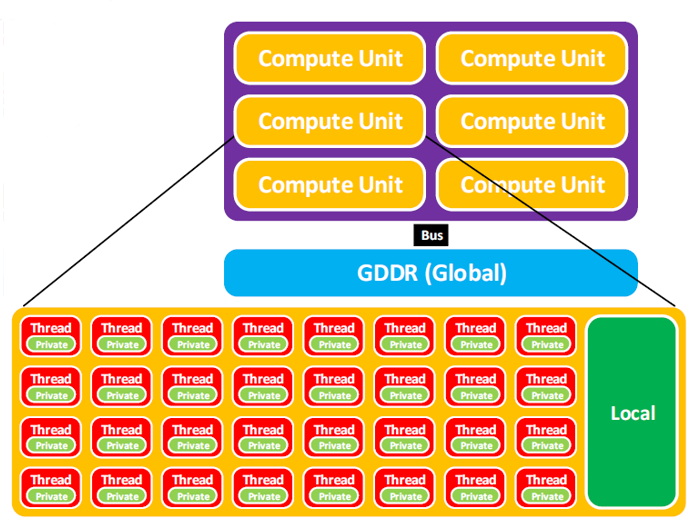
\includegraphics[width=0.7\textwidth]{figures/gpu_architecture.png}
\caption{GPU Architecture}
\end{figure}

\hypertarget{programming-heterogeneous-systems}{%
\subsection{Programming Heterogeneous
Systems}\label{programming-heterogeneous-systems}}

\begin{itemize}
\tightlist
\item
  C++ Accelerated Massive Parallelism (AMP)

  \begin{itemize}
  \tightlist
  \item
    open specification from Microsoft for implementing data parallelism
    directly in C++
  \end{itemize}
\item
  Compute Unified Device Architecture (CUDA)

  \begin{itemize}
  \tightlist
  \item
    parallel computing platform and programming model created by NVIDIA
    and implemented by the GPUs of NVIDIA
  \end{itemize}
\item
  OpenACC

  \begin{itemize}
  \tightlist
  \item
    programming standard for parallel computing developed by Cray, CAPS,
    NVIDIA, and PGI
  \end{itemize}
\item
  Open Computing Language (OpenCL)

  \begin{itemize}
  \tightlist
  \item
    C99 based language and framework for programming heterogeneous
    platforms
  \end{itemize}
\end{itemize}

\clearpage
\hypertarget{amp-overview}{%
\subsubsection{AMP Overview}\label{amp-overview}}

AMP code that cannot be run on GPUs will fall back onto one or more CPUs
instead and use SSE instructions

\begin{lstlisting}[language=C++]
#include <amp.h>
#include <iostream>
using namespace concurrency;

const int s = 5;
void vecadd() {
    int aH[] = {1, 2, 3, 4, 5};
    int bH[] = {6, 7, 8, 9, 10};
    int rH[s];

    //1 indicates the dimension of the vector. One could use up to 3 dimensions for a vector.
    array_view<const int, 1> a(s, aH);
    array_view<const int, 1> b(s, bH);
    array_view<int, 1> r(s, rH);
    r.discard_data(); //r should not be sent to the GPU. r is only meant to be the result vector.

    parallel_for_each(
        r.extent,
        [=](index<1> idx) restrict(amp)
    {
        r[idx] = a[idx] + b[idx];
    });
    // wait until the GPU has finished
    //and the result has been copied
    // back to rH
    r.synchronize();

    for (int i = 0; i < s; i++) {
        std::cout << rH[i] << "\n";
    }
}
\end{lstlisting}

\hypertarget{cuda-overview}{%
\subsubsection{CUDA Overview}\label{cuda-overview}}

CUDA gives program developers direct access to the virtual instruction
set and memory of the parallel computational elements in NVIDIA CUDA
GPUs. C/C++ programmers use `CUDA C/C++', compiled with ``nvcc''.

\begin{lstlisting}[language=C++]
//This code doesn't show how the data is transfered to the GPU. Instead, this code will be run directly on the GPU. The code identiefies on which thread it is running and gets the proper data (regarding the thread ID) out of the local computing memory.
__global__ void vecadd(int *a, int *b, int *r) {
    // get the workitem's unique ID
    const int idx = blockDim.x*blockIdx.x + threadIdx.x;
    // add two vector elements
    r[idx] = a[idx] + b[idx];
}
\end{lstlisting}

\clearpage
\hypertarget{openacc-overview}{%
\subsubsection{OpenACC Overview}\label{openacc-overview}}

Open Acc is designed to simplify parallel programming of heterogeneous
systems. Like in OpenMP, the programmer can annotate C, C++ and Fortran
source code to identify the areas that should be accelerated using
PRAGMA compiler directives.

\begin{lstlisting}[language=C++]
void vecadd(int *restrict r, int *a, int *b, int n) {
    #pragma acc kernels loop copyin(a[0:n],b[0:n]) copyout(r[0:n])
    for(int i = 0; i < n; ++i) r[i] = a[i] + b[i];
}
\end{lstlisting}

\hypertarget{introduction-to-opencl}{%
\subsection{Introduction to OpenCL}\label{introduction-to-opencl}}

Goal

\begin{itemize}
\tightlist
\item
  Use all computational resources in system (CPU \& GPU)
\item
  Efficient parallel programming model, based on C99
\end{itemize}

Kernel

\begin{itemize}
\tightlist
\item
  Basic unit of executable code - similar to a C function
\item
  A kernel is a function which is executed on the GPU
\end{itemize}

Program

\begin{itemize}
\tightlist
\item
  Collection of kernels and other functions
\item
  Analogous to a dynamic library
\end{itemize}

\begin{lstlisting}[language=OpenCL]
kernel void
dp_mul(global const float *a,
    global const float *b,
    global float *result)
{
    int id = get_global_id(0);
    result[id] = a[id] * b[id];
}
// execute dp_mul over "n" work-items
\end{lstlisting}

\begin{figure}[H]
\centering
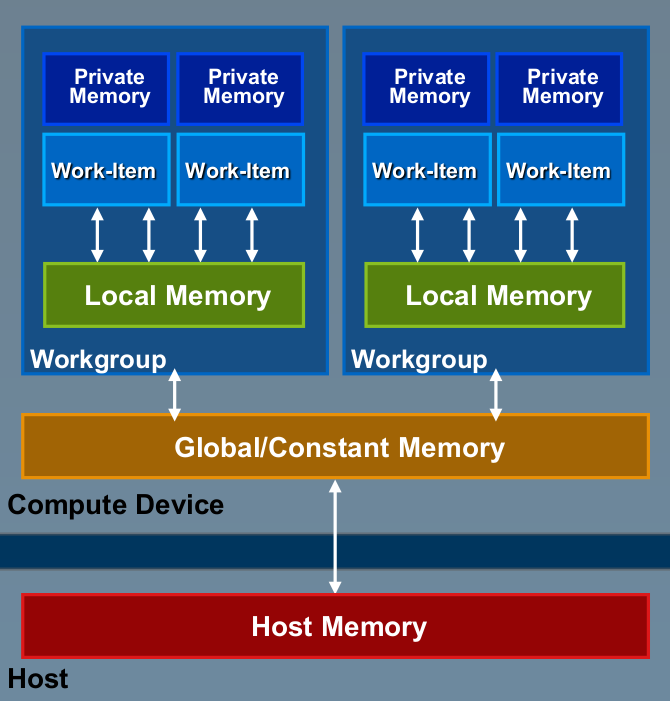
\includegraphics[width=0.5\textwidth]{figures/openClMemoryScheme.png}
\caption{OpenCL Memory Model}
\end{figure}

\begin{itemize}
\tightlist
\item
  Private Memory

  \begin{itemize}
  \tightlist
  \item
    Per Work-item
  \end{itemize}
\item
  Local Memory

  \begin{itemize}
  \tightlist
  \item
    Shared within a workgroup
  \end{itemize}
\item
  Local Global / Constant Memory

  \begin{itemize}
  \tightlist
  \item
    Not synchronized
  \end{itemize}
\item
  Host Memory

  \begin{itemize}
  \tightlist
  \item
    On the CPU
  \end{itemize}
\end{itemize}

\hypertarget{compilation}{%
\subsubsection{Compilation}\label{compilation}}

OpenCL uses dynamic compilation model (at runtime).

\begin{itemize}
\tightlist
\item
  Step 1 : The code is complied to an Intermediate Representation (IR),
  which is usually an assembler of a virtual machine.
\item
  Step 2: The IR is compiled to a machine code for execution. This step
  is much shorter.
\end{itemize}

\clearpage
\hypertarget{opencl-objects}{%
\subsubsection{OpenCL Objects}\label{opencl-objects}}

\begin{itemize}
\tightlist
\item
  Setup

  \begin{itemize}
  \tightlist
  \item
    Devices - GPU, CPU, Cell/B.E.
  \item
    Contexts - Collection of devices
  \item
    Queues - Submit work to the device (one task to CPU, one to GPU,
    etc.)
  \end{itemize}
\item
  Memory

  \begin{itemize}
  \tightlist
  \item
    Buffers - Blocks of memory
  \item
    Images - 2D or 3D formatted images (own data structures)
  \end{itemize}
\item
  Execution

  \begin{itemize}
  \tightlist
  \item
    Programs - Collections of kernels
  \item
    Kernels - Argument/execution instances
  \end{itemize}
\item
  Synchronization/profiling

  \begin{itemize}
  \tightlist
  \item
    Events
  \end{itemize}
\end{itemize}

\hypertarget{setup}{%
\subsubsection{Setup}\label{setup}}

\begin{enumerate}
\def\labelenumi{\arabic{enumi}.}
\tightlist
\item
  Get the device(s)
\item
  Create a context
\item
  Create command queue(s)
\end{enumerate}

\begin{lstlisting}[language=C++]
cl_uint num_devices_returned;
cl_device_id devices[2];
err = clGetDeviceIDs(NULL, CL_DEVICE_TYPE_GPU, 1, &devices[0], num_devices_returned);
err = clGetDeviceIDs(NULL, CL_DEVICE_TYPE_CPU, 1, &devices[1], &num_devices_returned);

cl_context context;
context = clCreateContext(0, 2, devices, NULL, NULL, &err);

cl_command_queue queue_gpu, queue_cpu;
queue_gpu = clCreateCommandQueue(context, devices[0], 0, &err);
queue_cpu = clCreateCommandQueue(context, devices[1], 0, &err);
\end{lstlisting}

\clearpage
\begin{itemize}
\tightlist
\item
  Devices

  \begin{itemize}
  \tightlist
  \item
    Multiple cores on a CPU or a GPU are presented as a single device
  \item
    OpenCL executes kernels across all cores in a data-parallel manner
  \end{itemize}
\item
  Contexts

  \begin{itemize}
  \tightlist
  \item
    Enable sharing of memory between devices
  \item
    To share between devices, both devices must be in the same context
  \end{itemize}
\item
  Queues

  \begin{itemize}
  \tightlist
  \item
    All work submitted through queues
  \item
    Each device must have a queue
  \end{itemize}
\end{itemize}

\hypertarget{read-and-write}{%
\subsubsection{Read and Write}\label{read-and-write}}

\textbf{Read from a region in memory object to host
memory}

\begin{lstlisting}[language=C++]
clEnqueueReadBuffer(queue, object, blocking, offset, size, *ptr, ...)
\end{lstlisting}

\textbf{Write to a region in memory object from host memory}

\begin{lstlisting}[language=C++]
clEnqueueWriteBuffer(queue, object, blocking, offset, size, *ptr, ...)
\end{lstlisting}

\hypertarget{data-types}{%
\subsubsection{Data Types}\label{data-types}}

\begin{itemize}
\tightlist
\item
  Scalar data types

  \begin{itemize}
  \tightlist
  \item
    char , uchar, short, ushort, int, uint, long, ulong
  \item
    bool, intptr\_t, ptrdiff\_t, size\_t, uintptr\_t, void, half
    (storage)
  \end{itemize}
\item
  Image types

  \begin{itemize}
  \tightlist
  \item
    image2d\_t, image3d\_t, sampler\_t
  \end{itemize}
\item
  Vector data types

  \begin{itemize}
  \tightlist
  \item
    Portable
  \item
    Vector length of 2, 4, 8, and 16
  \item
    char2, ushort4, int8, float16, double2, \ldots{}
  \item
    Endian safe
  \item
    Aligned at vector length
  \item
    Vector operations and built-in functions
  \end{itemize}
\end{itemize}

\clearpage
\hypertarget{programming-in-opencl}{%
\subsubsection{Programming in OpenCL}\label{programming-in-opencl}}

In General: 3 Major Code Blocks

\begin{itemize}
\tightlist
\item
  OpenCL device program: kernels and subroutines

  \begin{itemize}
  \tightlist
  \item
    operations executed by the work items
  \item
    C99 based syntax with vector operations
  \end{itemize}
\item
  C++ host program: device and kernel preparation (reusable)

  \begin{itemize}
  \tightlist
  \item
    platform and device handling
  \item
    creating contexts and command queues
  \item
    compiling OpenCL device programs
  \end{itemize}
\item
  C++ host program: data and device program enqueing

  \begin{itemize}
  \tightlist
  \item
    data allocation and management
  \item
    filling in command queues
  \item
    setting kernel arguments
  \item
    running kernels
  \item
    event handling
  \end{itemize}
\end{itemize}

\hypertarget{opencl-example-vector-addition}{%
\subsection{OpenCL Example: Vector
Addition}\label{opencl-example-vector-addition}}

??

\clearpage